\section{Basic concepts}


%%=============================================================================
\subsection{logarithms}


\begin{df}[Logarithms]
    Let $a,b$ be two positive real numbers, 
    and $a \neq 1$. 
    \textit{The logarithm of $b$ to the base $a$},
    denoted by {\color{purple} $\log_a b$}, 
    is the unique real number $x$ such that $a^x = b$. 
    % 
    That is, 
    \[
        \log_a b = x \quad \text{iff} \quad a^x = b.
    \]
\end{df}

The logarithm function is the inverse of the exponential function. 
% 
The logarithm function is defined for $a>0$, $a \neq 1$, and $b>0$. 
% 
The most commonly used bases are $a=2$, $a=e$, and $a=10$. 
% 
The base $a=2$ is used in computer science, 
$a=e$ is used in calculus, 
and $a=10$ is used in engineering and science. 
The base $a=10$ is called the \textit{common logarithm}, 
and is denoted by $\lg b$.

\begin{table}[ht!]
    \centering
    \caption{Commonly used bases for logarithms}
    \label{tab: logarithm}
    \vspace{1em}
    \begin{tabular}{c||c}
        \hline
        Base & Notation \\
        \hline
        $2$ & {\color{purple} $\log b$} \\
        $e$ & $\ln b$ \\
        $10$ & $\lg b$ \\
        \hline
    \end{tabular}
\end{table}

$\log_a b \quad\leadsto\quad  a^\Box = b$

$e \approx 2.718$

\begin{table}[h]
    \centering
    \renewcommand{\arraystretch}{1.3} % 行距
    \caption{Identities of logarithms}
    \vspace{1em}
    \begin{tabular}{c||l}
    \hline
    Identity & \multicolumn{1}{c}{Formula}  \\
    \hline
    
    Product & $\log_b(xy) = \log_b x + \log_b y$ \\

    Quotient & $\log_b(\frac{x}{y}) = \log_b x - \log_b y$ \\

    Power & $\log_b x^r = r \cdot \log_b x$ \\

    Root & $\log_b \sqrt[r]{x} = \frac{1}{r} \cdot \log_b x$ \\
    \hline
\end{tabular}
\end{table}






% figure
\begin{figure}[ht!]
    \centering
    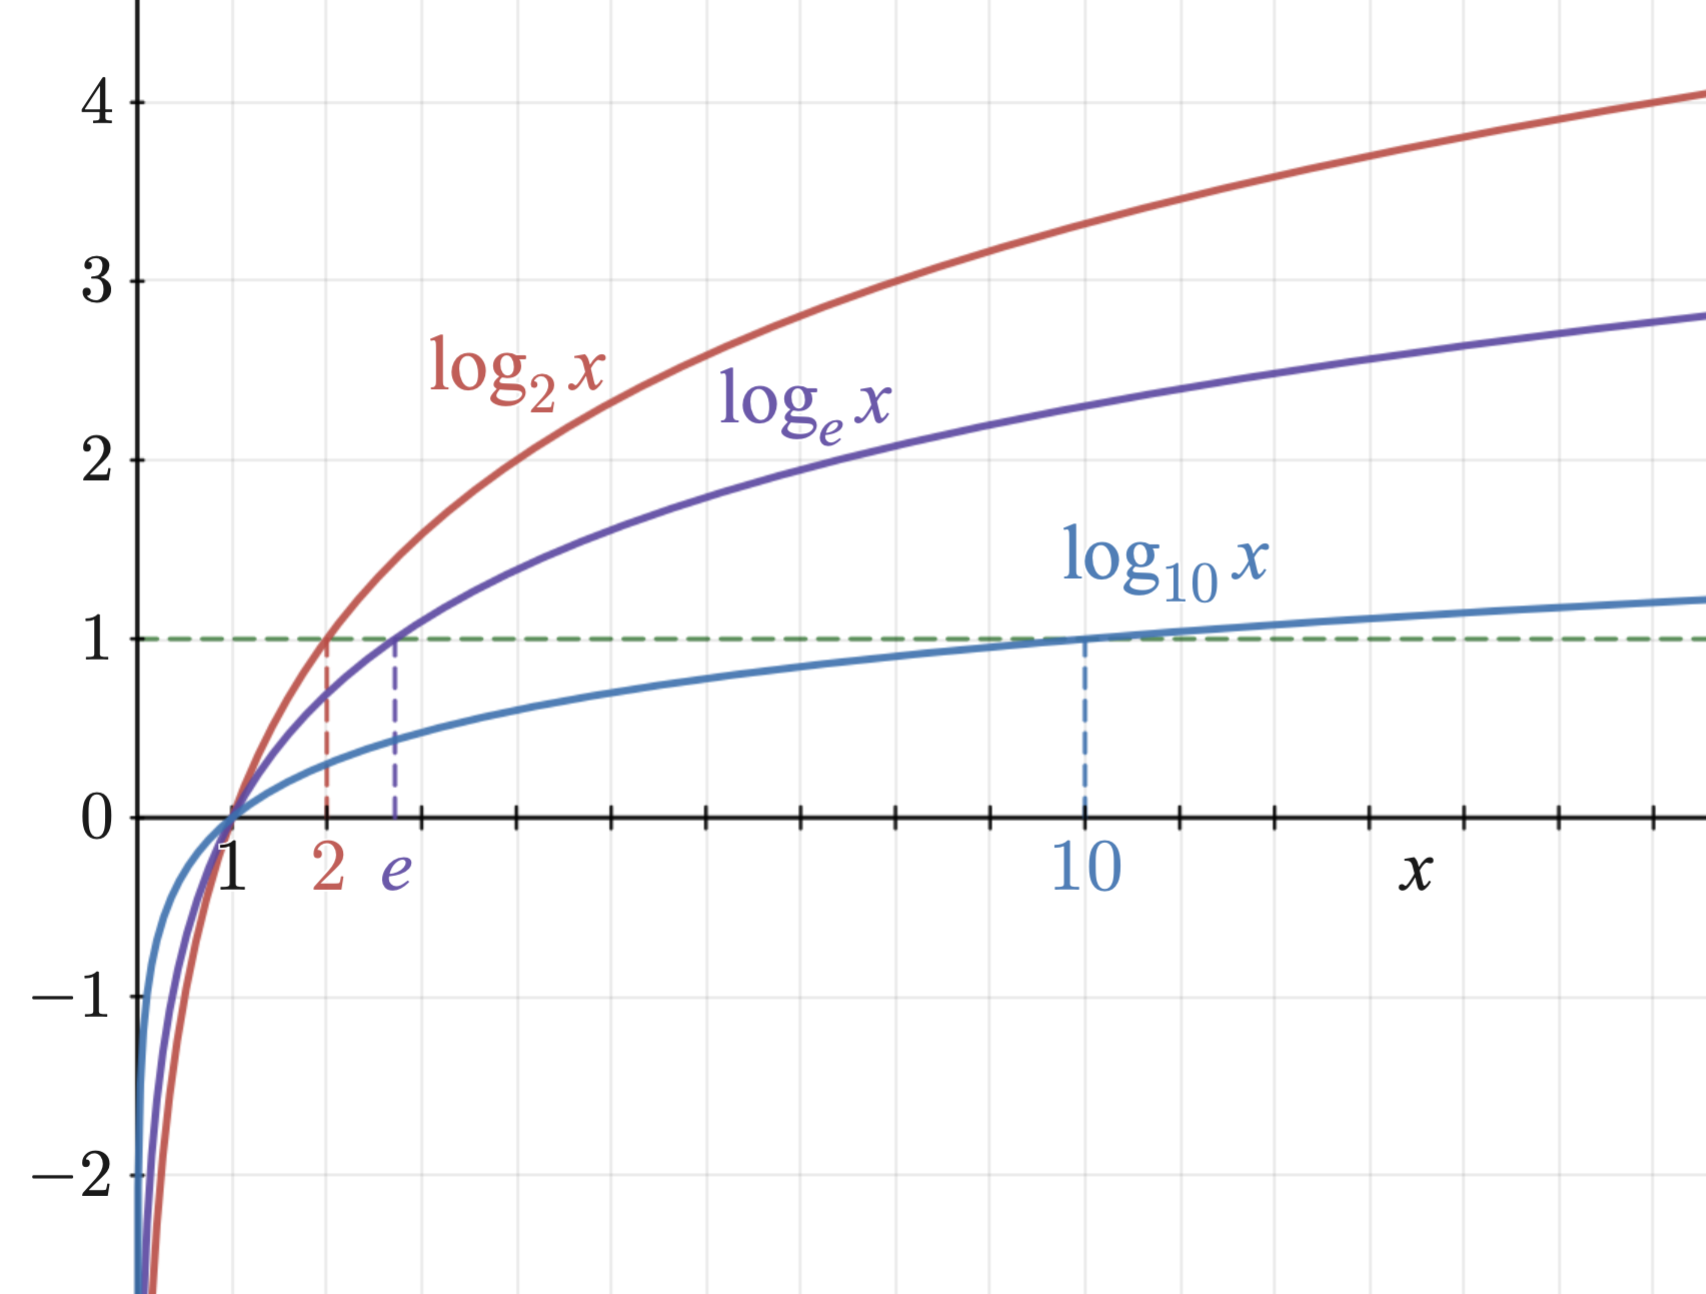
\includegraphics[width=.5\textwidth]{fig/logarithm.png}
    \caption{Plots of logarithm functions, with three commonly used bases, from \href{https://en.wikipedia.org/wiki/Logarithm}{wikipedia}}
    \label{fig: logarithm}
\end{figure}





%%=============================================================================
\subsection{Strings}

If $S$ is a \textit{finite} set, called \textit{alphabet set}, 
then a \textit{string} over $S$ is a finite ordered tuple of elements from $S$. 

We will typically consider the \textit{binary} alphabet $2 = \{0,1\}$.


$S^0 = \{\epsilon\}$

$S^* = \bigcup_{n \geq 0} S^n$ is the set of all strings over $S$.


The \textit{concatenation} of strings $x,y$ is denoted by $x^\frown y$, $x \circ y$, or simply $xy$.


$x^k$ denotes the concatenation of $k$ copies of $x$ for $k \geq 1$. 
% 
For example, 
$1^3$ is `$111$'.

The length of a string $x$ is denoted by $|x|$.


%%=============================================================================
\subsection{Representations}


we implicitly identify any function $f$ whose domain and range are not strings with the function 
\[
    g \colon \{0,1\}^* \to \{0,1\}^*
\]
that given a representation of an object $x$ as input, 
outputs the representation of $f (x)$. 


%%=============================================================================
\subsection{Big--Oh notation}



\begin{df}[Big--Oh notation]
    If $f,g$ are two functions over $\mathbb{N}$, 
    then we say that 
    \begin{enumerate}[itemsep=5pt,parsep=5pt,leftmargin=3em,topsep=5pt,label=(\arabic*)] %% or label = \alph*, \roman*
        \item 
        {\color{purple} $f = O(g)$} if there exist a constant $c$ such that $f(n) \leq c \cdot g(n)$ for every sufficient large $n$.

        \item 
        $f = \Omega(g)$ if $g = O(f)$.

        \item 
        $f = \Theta (g)$ if $f=O(g)$ and $g=O(f)$.

        \item 
        {\color{purple} $f=o(g)$} if for $\forall \kappa > 0$, 
        $f(n) \leq \kappa \cdot g(n)$ for every sufficient large $n$.

        \item 
        $f = \omega(g)$ if $g = o(f)$.
    \end{enumerate}   

    To emphasize the input parameter, 
    we often write {\color{purple} $f(n)=O(g(n))$} instead of $f= O(g)$, 
    and use similar notation for $o,\Theta,\Omega,\omega$.
\end{df}



\begin{example}
    Here are some examples of big--Oh notation:
    \begin{enumerate}[itemsep=5pt,parsep=5pt,leftmargin=3em,topsep=5pt,label=(\arabic*)] %% or label = \alph*, \roman*
        \item 
        If $f(n)=100n\log n$ and $g(n)=n^2$, 
        then $f = O(g)$.

        \item 
        If $f(n) = 100n^2 + 24n + 2\log n$ and $g(n)=n^2$, 
        then $f=O(g)$ and $g=O(f)$.
    \end{enumerate}
\end{example}



